%! TeX program = lualatex
\documentclass[]{beamer} 

\setbeamercolor{title}{fg=black}
\setbeamercolor{frametitle}{fg=black}
\setbeamercolor{caption}{fg=black}
\setbeamercolor{caption name}{fg=black}

\setbeamertemplate{navigation symbols}{}
\setbeamertemplate{itemize item}{\color{black}$\bullet$}

% packages
\usepackage{fontspec}
\setmainfont{EB Garamond}
\usefonttheme{serif}
\setmonofont[Scale=MatchLowercase]{Deja Vu Sans Mono}

\usepackage{microtype}      % Slightly tweak font spacing for aesthetics
\usepackage[english]{babel} % Language hyphenation and typographical rules

\usepackage{minted}
\usemintedstyle{algol_nu}
\usepackage{xcolor}

\usepackage{pgfplots}
\pgfplotsset{width=\textwidth,compat=1.9}

\usepackage{caption}
\newenvironment{code}{\captionsetup{type=listing, skip=0pt}}{}

\usepackage[yyyymmdd]{datetime}
\renewcommand{\dateseparator}{--}

\usepackage{titlesec}

\author{Andrew Hayes (ID: 21321503)}
\title{Why Vim is My Favourite Text Editor}
\subtitle{CT3112 Professional Skills: Assignment 01}
\institute{University of Galway}

\begin{document}

\titlegraphic{
\includegraphics[width=3cm]{./images/vim_logo.png}}
\frame{\titlepage}

\begin{frame}{Introduction}
    By the end of this presentation, I intend for you to have gained an understanding of:
    \begin{itemize}
        \item   What Vim is.
        \item   The benefits of Vim.
        \item   The drawbacks of Vim.
        \item   Why I prefer Vim for all my text-editing work.
        \item   Whether or not Vim might be the right text editor for you.
    \end{itemize}
\end{frame}

\begin{frame}{What is Vim?}
    \begin{itemize}
        \item   \textbf{Vim} is terminal-based, modal text editor released in 1991, designed to be minimal \& fast to
                use.
        \item   It has a number of fast, mnemonic keybindings that make typical text-editing tasks much faster.
        \item   A \textbf{terminal-based} text editor is a text-only editor that is ran from the command line or
                terminal.
        \item   A \textbf{modal} text editor is one in which there are a number of different \textbf{modes} that the 
                editor can be in at any one time. 
    \end{itemize}
\end{frame}

\begin{frame}
    \begin{figure}[h]
        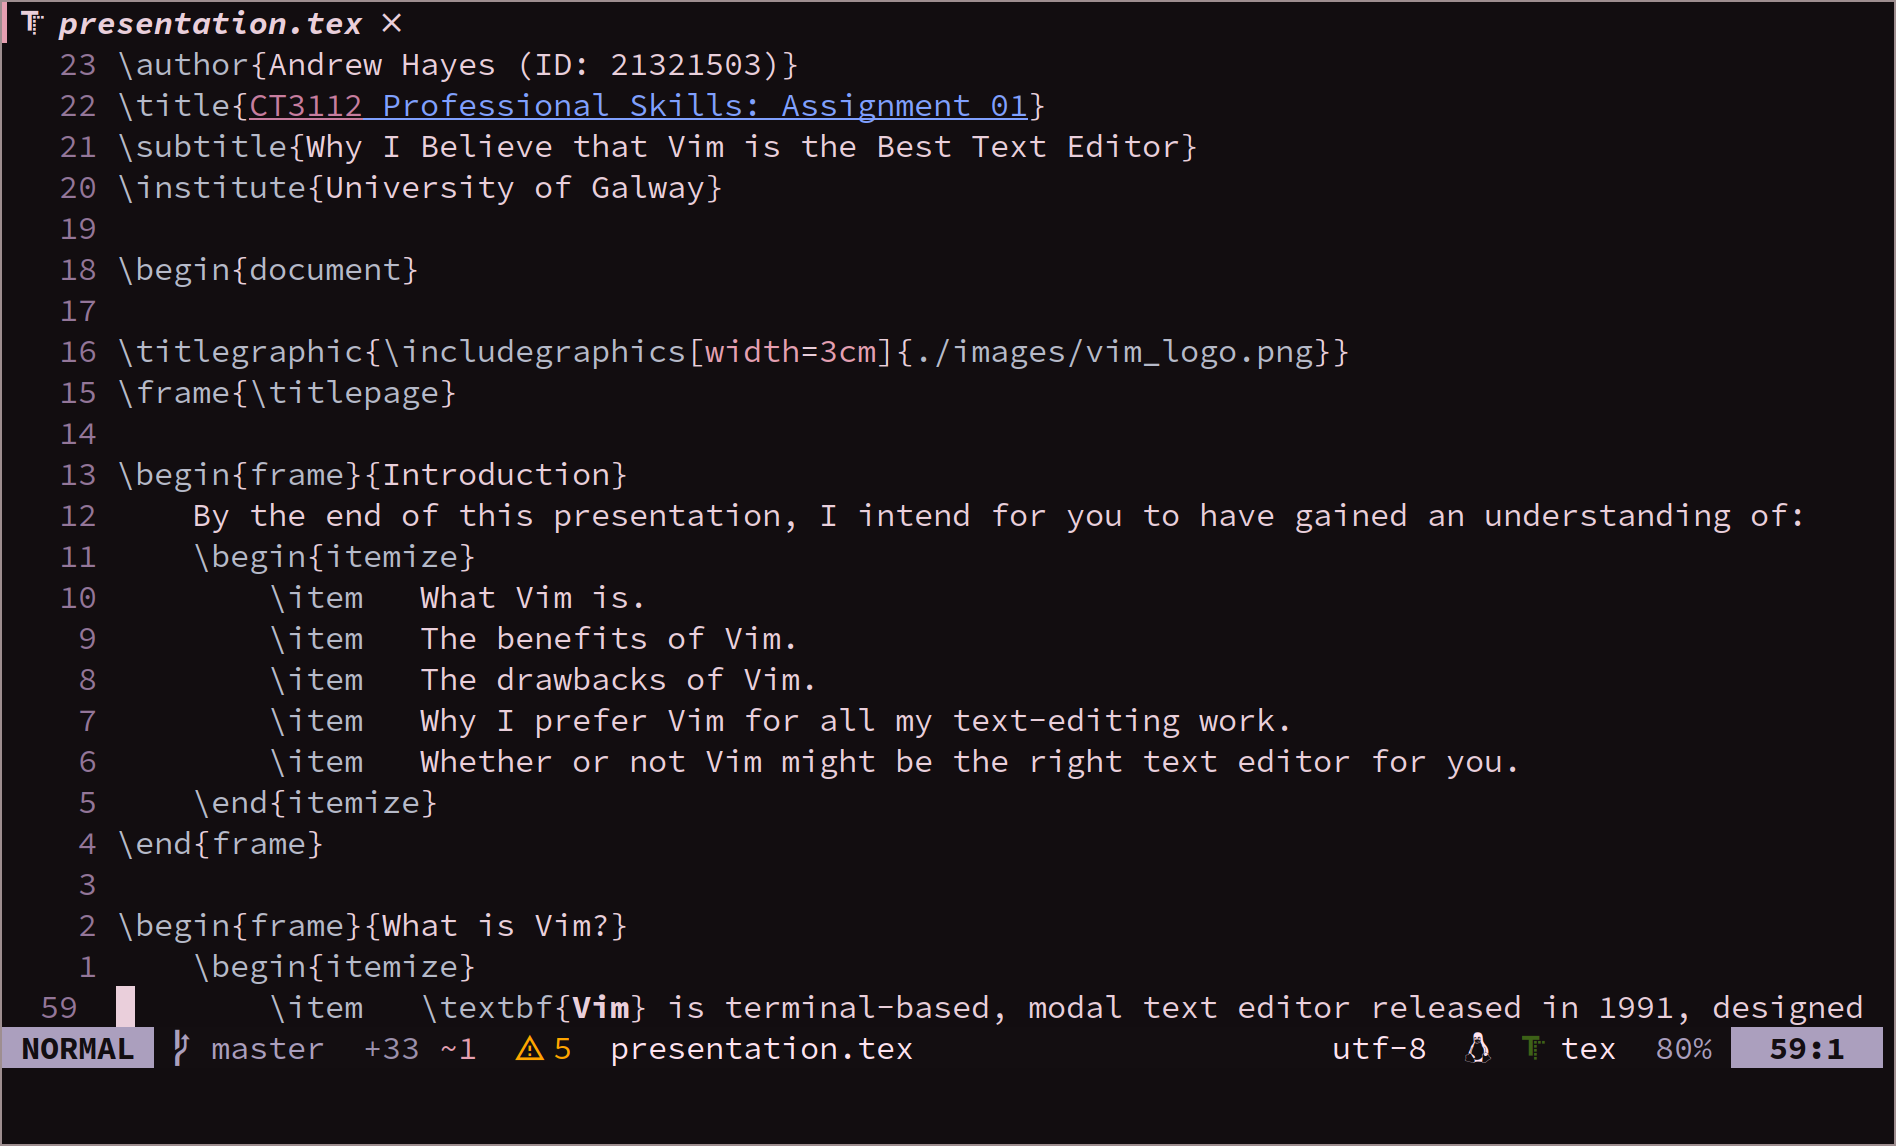
\includegraphics[width=\textwidth]{./images/screenshot.png}
        \caption{A Screenshot of Vim Being Used to Write this Presentation (in {\LaTeX})}
    \end{figure}
\end{frame}

\begin{frame}{What is a Terminal?}
    \begin{itemize}
        \item   A \textbf{terminal} is a text-based interface for a computer, originating from when computers did not
                have any graphics.
        \item   It is typically interacted with via a \textbf{command line}, where text commands are written to start
                programs.
        \item   To start Vim from the command line, simply type \mintinline{bash}{vim file_name.txt}
    \end{itemize}

    \begin{figure}[h]
        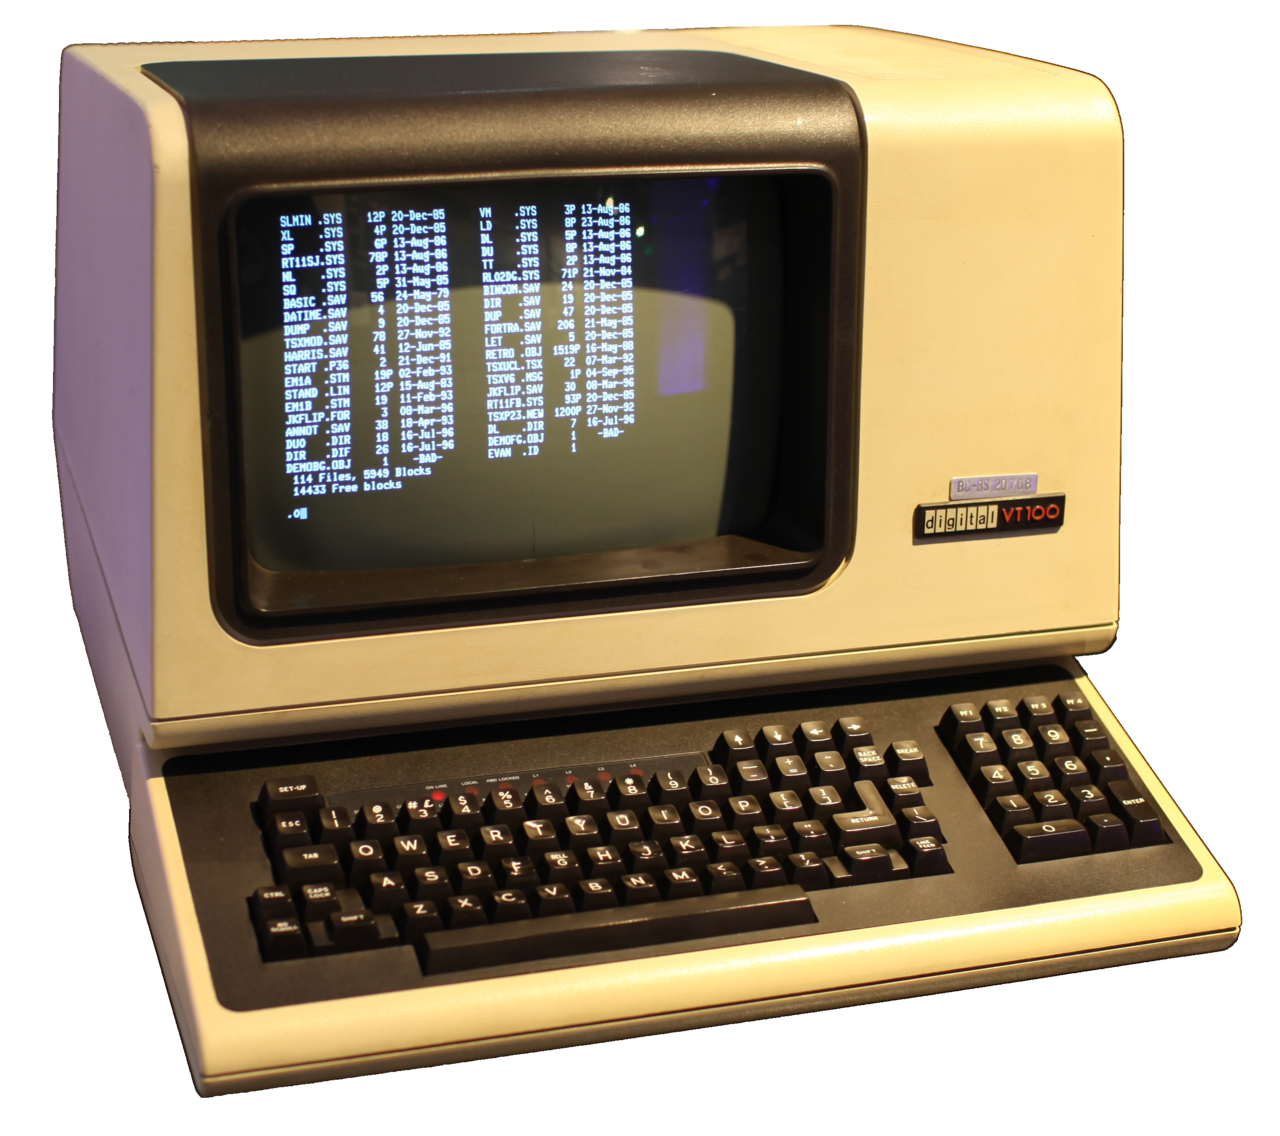
\includegraphics[width=0.4\textwidth]{./images/terminal.png}
        \caption{A Computer Terminal from 1978}
    \end{figure}
\end{frame}

\begin{frame}{What are the Vim Modes?}
    \begin{itemize}
        \item   \textbf{Normal mode} (\texttt{ESC}) is for the navigation \& manipulation of the text in the file
                being edited, via the shortcut keybindings.
                It is the default mode of the program.
        \item   \textbf{Insert mode} (\texttt{i}) is for inserting new text. This mode is similar to the
                default to the default behaviour of a more traditional text editor such as Notepad: text can be typed
                or removed with the backspace key, and navigation or selection can be done with the mouse or arrow
                keys.
        \item   \textbf{Visual mode} (\texttt{v}) is for the selection of text blocks for manipulation, with the
                selected text being highlighted, similar to selecting text with the mouse in other text editors.
                Visual mode has two sub-modes: \textbf{visual block} (\texttt{CTRL+v}) \& \textbf{visual line}
                (\texttt{V}), in which text can be selected either vertically by columns or horizontally by line.
    \end{itemize}
\end{frame}

\begin{frame}{What are the Vim Keybindings?}
    \begin{itemize}
        \item   Too many to list here!
        \item   Navigation in normal mode can be done with the \texttt{hjkl} (direction) keys, which correspond to
                the left, down, up, \& right arrow keys respectively, allowing quick navigation without removing your
                fingers from the home row.
    \end{itemize}
\end{frame}


\end{document}
